% History
% 12/06/2024  (岸)	修論下書き用texファイル作成
% 12/12/2024  (岸)	フォントサイズを11pt, 行間を1.5に設定
% コンパイルの仕方
% 		uplatex chapter1_v1.tex
% 		upbibtex chapter1_v1
% 		uplatex chapter1_v1.tex
% 		uplatex chapter1_v1.tex
% 		dvipdfmx chapter1_v1.dvi

% フォントサイズを11ptに設定
\documentclass[a4paper,11pt,nomag]{jsreport}

\usepackage[dvipdfm,truedimen]{geometry}
\geometry{top=22mm,bottom=22mm,left=22mm,right=22mm}
%% jsclasses系で文字サイズ11pt や 12pt をクラスオプションに指定すると,
%% 長さが拡大されるため,nomagオプションを併用している.
%% https://oku.edu.mie-u.ac.jp/~okumura/jsclasses/ のFAQをよく読むこと.

%\usepackage{layout}
%\usepackage[utf8]{inputenc} %不要かも
\usepackage[T1]{fontenc} %utf8フォントエンコーディング指定
\usepackage{lmodern} % 11pt, nomag を使っているので
% CloudLaTeX の場合は下の1行を有効にすること
% \AtBeginDvi{\special{pdf:mapfile ptex-ipaex.map}}
\usepackage{array}
\newcommand{\bhline}[1]{\noalign{\hrule height #1}}  
\newcommand{\bvline}[1]{\vrule width #1}
\renewcommand{\baselinestretch}{1.5} % 教授が赤修正を入れやすいように行間を1.5に設定
\usepackage[singlespacing]{setspace} % 部分的な行間調整パッケージ.表など行間を1.5倍にしたくないところに使う.
\usepackage[subrefformat=parens]{subcaption}
\usepackage[dvipdfmx]{graphicx} % dvipdfmx を前提としている
\usepackage[dvipdfmx]{color}
\usepackage{caption}
\usepackage{subcaption}
\usepackage{multirow}
\usepackage{arydshln}
\usepackage{here} % 図表の位置決め用
\usepackage{amsmath,amssymb}% 数式用
\usepackage{bbm}
\usepackage{bm} % 数式太字
\usepackage{url}      % URL等記載用.\verbより便利
\usepackage{enumerate}
\usepackage{midpage}
% ハイパーリンク
\usepackage[dvipdfmx,breaklinks=true,colorlinks]{hyperref} % dvipdfmxは日本語のときのみかく
\usepackage{pxjahyper} % (u)pLaTeXのときのみかく

% サブキャプションのフォーマットを調整
\renewcommand\thesubfigure{(\alph{subfigure})}
\captionsetup[subfigure]{labelformat=simple, labelsep=space}

\begin{document}
\setcounter{chapter}{2}

\chapter*{深層学習を用いた動物分類に関する既存研究}

\section{赤外線画像に対する動物分類に関する既存研究}

気候変動や人口増加が生態系に与える影響を把握し,野生動物と人間の持続可能な共存を実現することは重要な課題である.
この課題を解決するため,生態系モニタリングの重要性が世界的に高まっている \cite{zwerts2021, bandaru2024}.
生態系モニタリングの手法として,監視カメラなどを用いた観測が広く採用されており,特定地域における動物種の個体数推定だけでなく,環境に対する各動物種の生態観察や研究が行われている \cite{trolliet2014}.
特に,カメラトラップは,観察者による直接的な介入を最小限に抑えることが可能であり,観察者の存在が個体の行動に与える影響を軽減することができるため,
野生動物の監視ツールとして広く活用されている \cite{本郷2018, abood2023}.
カメラトラップは,赤外線センサなどを用いた自動撮影により人的労力を削減することができ,近年のデジタルカメラの高性能化に伴い長期間にわたる連続的なモニタリングが可能である.
一方で,カメラトラップを使用した生態系モニタリングでは,複数箇所にカメラトラップを設置するため膨大な画像枚数を取得することも多く \cite{kays2020, si2014},
記録された画像・動画中に対する人手による動物の有無や種の推定は多大なアノテーションコストを要する \cite{thangaraj2023}.
加えて,種の分類には専門的な知識が必要であることも作業員確保によるコスト面での課題である.
さらに,技術革新は今後も進むと予想されるのに対し,アノテーションコストを著しく下げることは困難であるため,このギャップは今後一層拡大していくと予想される \cite{安藤2019}.
したがって,これらの課題を解決するため,カメラトラップによって撮影された画像・動画中から自動で動物を検出・識別する手法の実現が望まれている.

近年では,画像処理技術と機械学習を用いた野生動物の自動識別手法が研究されている \cite{manna2023, mohanty2022}.
国際的な画像認識アルゴリズム性能コンペティションとして知られるImageNet Large Scale Visual Recognition Challenge (ILSVRC)の2012年大会において,
AlexNet \cite{alexnet}が画期的な成功を収めて以降,画像処理分野の様々なタスクにおいてCNNに基づく手法が盛んに研究されている \cite{mohanty2016, sue2020}.
また,その多くのタスクでCNNは高い性能を実現しており,カメラトラップによる動物識別に関する研究においてもCNNを用いた手法がいくつか提案されている \cite{agarwal2023, neeli2023, thangaraj2023, abood2023}.
Tanら \cite{tan2022}は,2014年から2020年にかけて撮影された約25,000枚の自作データセットを用いて,YOLO-V5 \cite{yolov5},FCOS(Fully Convolutional One-Stage Object Detection) \cite{fcos},
Cascade R-CNN \cite{cascade}の3つの検出ネットワークでの比較検証,および映像に適用した動物認識の性能を評価している.
Tabakら \cite{tabak2019}は,全米5箇所で撮影された約300万枚のカメラトラップ画像を用いて,独自のCNNにより動物の画像分類を行っている.

しかしながら,上記のような既存研究の分類モデルを学習するために用いられた大規模なデータセットは,多くの撮影場所や数年間に及ぶ長期間の撮影によって蓄積された画像で構成されている.
したがって,これらの既存研究は,個人的な利用での撮影や狭い範囲の地域での撮影など,十分な画像データを収集できない状況には適していないため、実用面での課題が残る.
また,夜間に行動する動物の撮影には赤外線カメラを用いることが有効であるが,赤外線カメラで撮影された画像は色情報を含まないなど,可視光カメラで撮影された画像とは映り方が異なる.
したがって,真に実用的な生態系モニタリングシステムの実現に向けて,赤外線カメラによって撮影された少数の学習用データから,効果的に学習可能な深層学習モデルの開発が急務である.

このような既存研究の課題解決に向けた研究として,少数の赤外線画像を用いた動物分類が検討されている.
Kishiら \cite{kishimoto2023}は,米国南西部の140箇所で撮影された画像3,000枚を用いて,CNNによる少数の赤外線画像を用いた動物分類を行っている.
この先行研究では,少数データを用いた効率的な深層学習モデルの学習を目的とするFSLの分野において有効な手法である転移学習とデータ拡張の赤外線画像に対する有効性が検証された.
まず,転移学習は,事前に大量のデータを用いて学習したモデルを新しいタスクに適用する手法である.
この先行研究では,画像認識タスクで一般的に用いられるImageNetデータセット,ImageNetデータセットを擬似赤外線化した画像,
さらに数式から生成されたフラクタル画像による転移学習の有効性が検証された.
一方,データ拡張については,一般的な幾何学変換や色変換などの画像変換に加え,画像の一部をマスクし隠すことでモデルの汎化性能を向上させるRandom Erasingや,
複数の画像処理を組み合わせることで新しい画像を生成しモデルの頑健性を向上させるAugmixなどの有効性が検証された.
実験の結果,転移学習では疑似赤外線画像,フラクタル画像,ImageNetの順に効果が高いことが示され,データ拡張についてはAugMixが特に有効であることが明らかになった.

Kishiらの研究では,新規地域に対する深層学習モデルの適用開始時の状況を想定しており,学習に使用する画像は1クラスあたり50枚としている.
しかし,実運用を想定すると1クラスあたり50枚程度の画像収集すら困難な場合も考えられる.
また,評価実験における評価用データセットでは学習用データセットと同じ動物種のみが使用されており,モデルの適用地域に生息する全ての動物種がモデルに登録されている閉集合が仮定されている.
しかし,モデルの実運用開始時において,対象地域に生息する全ての動物種のデータを網羅的に収集することは現実的ではない.
従来の分類モデルでは,学習データに含まれないモデルに未登録の動物を正しく識別できず,登録済みのクラスに強制的に分類されてしまうオープンセット問題が存在する.
図 \ref{fig:non_osr}は,従来の分類モデルが未登録の動物を識別できない例を示している.
% 
\begin{figure}[tbp]
  \centering
  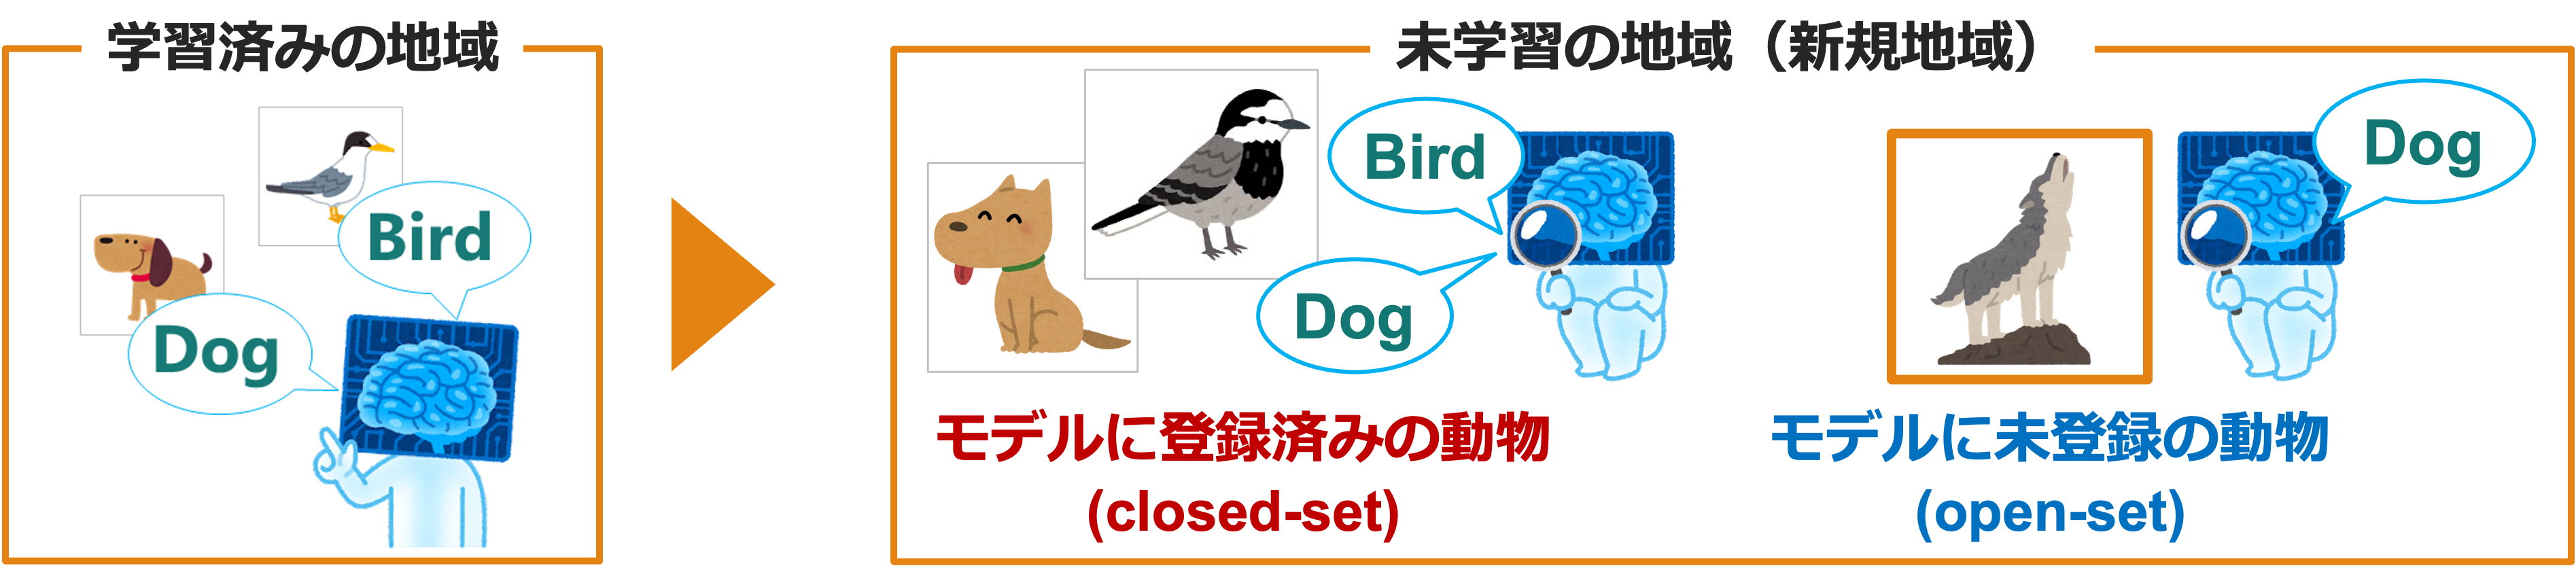
\includegraphics[width=\linewidth, keepaspectratio]{image/non_osr.png}
  \caption{従来の分類モデルによるオープンセット問題の例}
  \label{fig:non_osr}
\end{figure}
% 
図 \ref{fig:non_osr} に示される通り,犬と鳥のみを学習したモデルを新規地域に適用した場合,モデルに登録済みの犬や鳥は分類できるが,未登録の動物であるオオカミは登録済みの動物種に強制的に分類されてしまう.
このような誤分類はモデルの精度低下へと繋がるため,未登録の動物種を適切に検出できるOSRモデルの開発が急務となっている.
なお,本論文では,モデルに登録されているクラスセットをクローズドセット(closed-set),モデルに未登録のクラスセットをオープンセット(open-set)と呼ぶ.


\section{Few-Shot Open-Set Recognitionに関する既存研究}

昨今の第3次AIブームにおける機械学習システムの高い性能や実用的な成果は,主にクローズドセットタスクにおいて達成されてきた.
これらのシステムでは,学習用データセットと評価用データセットに同一のクラスが含まれることを前提としており,システムの評価は学習時に登録されたオブジェクトクラスのみを対象として実施される.
しかしながら,より実用的なシステムの実現を目指す場合,現実的な問題設定としてオープンセット問題への対応が不可欠である \cite{geng2021survey}.
機械学習ベースのシステムの利用が進むにつれ,幅広いアプリケーションにおいて高い頑健性を備えた手法が要求されており,OSR技術に注目が集まっている \cite{sun2023survey}.
OSRは,学習時に想定していないクラスのデータが入力された場合でも,システムを頑健に機能させるためのアプローチの1つとして位置付けられている.
図 \ref{fig:osr}にOSRにおける未登録データの検出プロセスの一例を示す.
% 
\begin{figure}[tbp]
  \centering
  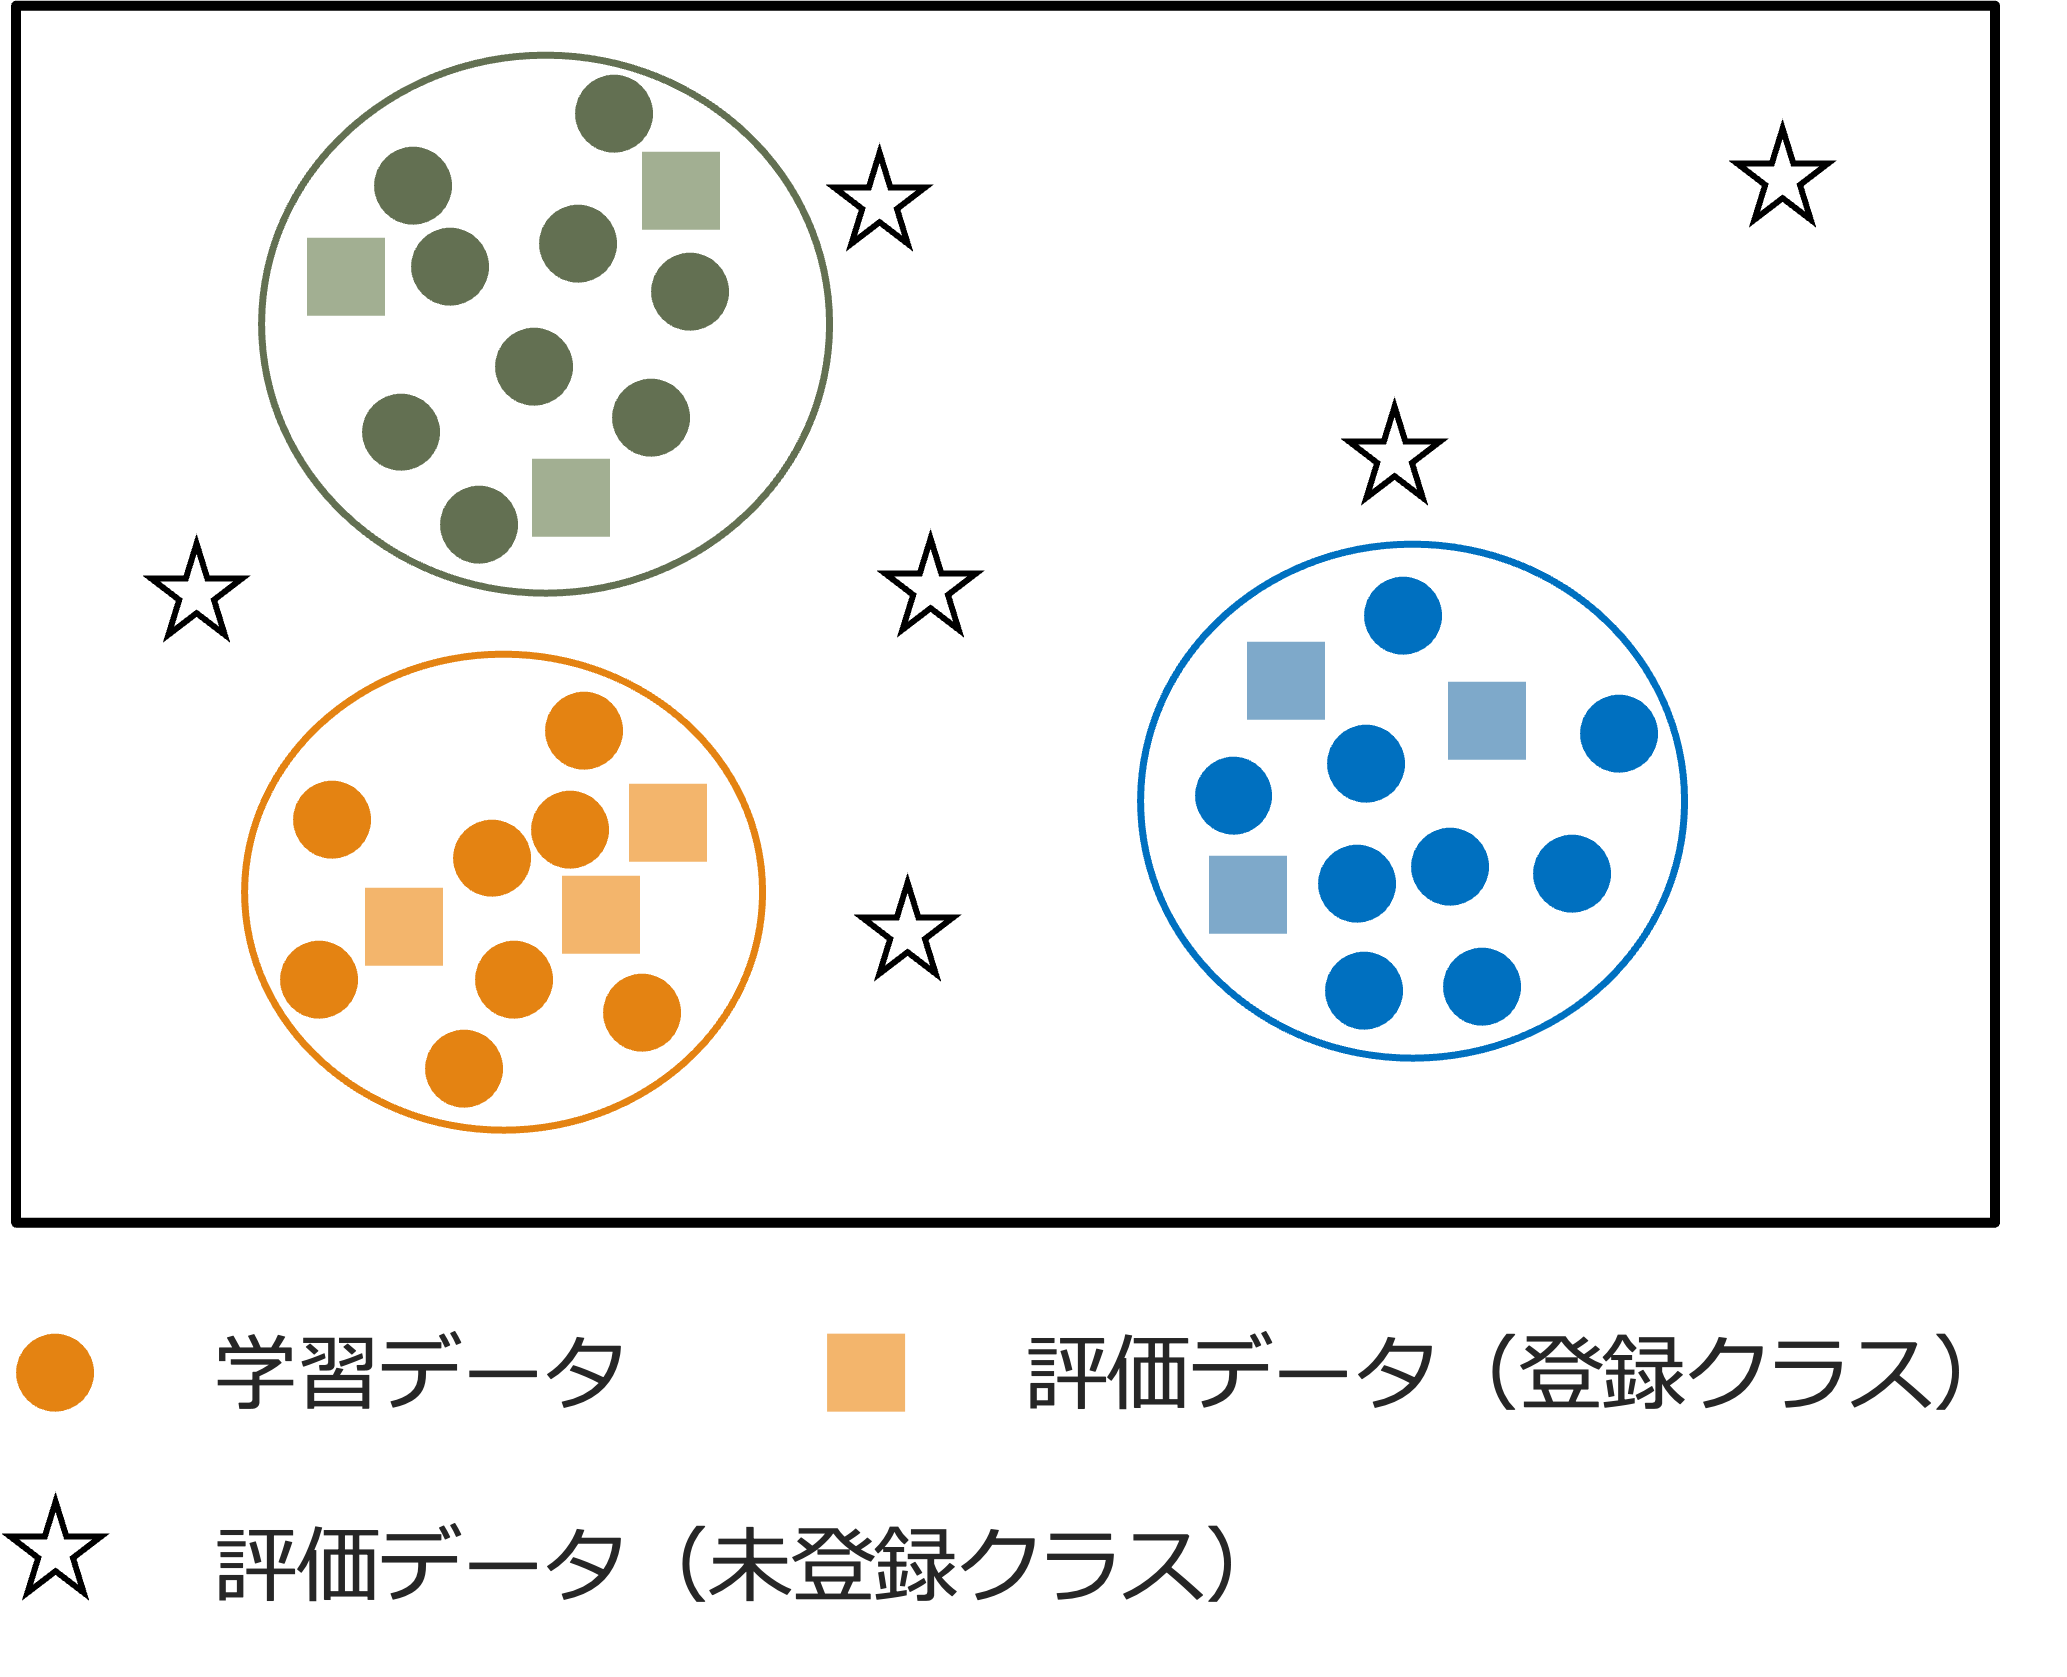
\includegraphics[width=0.6\linewidth, keepaspectratio]{image/osr.png}
  \caption{OSRにおける未登録データの検出プロセスの一例}
  \label{fig:osr}
\end{figure}
% 
既存の分類モデルでは未登録データを既存クラスに分類してしまう課題があったが,分類対象の画像の特徴量と既存クラスの類似度が特定の閾値を下回る場合に未登録クラスとして検出することで,
この課題を解決することが可能となった.

実世界における動的な環境下での認識・分類タスクに対して,\textcolor{red}{より実用的な}モデルを構築するためには未登録クラスへの対応が不可欠である.
% これを考慮しない場合,システムの不適切な開発につながり,その有用性が著しく制限されることとなる.
しかし,学習時に想定されていないクラスは無数に存在する可能性があり,それらすべてを事前に予測して学習データに含めることは現実的ではない \cite{mahdavi2021survey}.
特に,深層学習モデルはデータ駆動型のアプローチのため,適切な帰納バイアスを獲得するために大量の学習データを必要とする.
同様に,既存のOSR手法においても大量の学習データの利用を前提としており,その適用範囲は局所的な場面に限定されている \cite{wang2023}.

この課題に対し,近年ではFew-Shot Open-Set Recognition(FSOSR)という新たな研究分野が注目を集めている \cite{peeler, che2023}.
FSOSRは,少数の画像データからの効率的な学習による正確な分類を行うことと,学習データに存在しないデータを未登録クラスとして検出・拒絶できるモデルの構築を目的とした研究分野である.

Jeongら \cite{snatcher}は,変換一貫性(transformation consistency)という概念に基づき,未登録クラスを検出するSnaTCHerを提案した.
これは,類似した入力データは特徴空間での変換後も近い位置関係を保つという性質を利用している.
未登録クラスの入力データは,登録クラスとは異なる特徴空間を形成する傾向があるため,変換後の特徴量は登録クラスのプロトタイプから大きく離れることが期待される.
プロトタイプとは,登録クラスを代表する特徴ベクトルのことであり,登録クラスから得られた特徴量の平均値を求めることによって生成される.
この手法の最大の利点は,疑似的な未登録クラスサンプルを必要としない点である.
OSRなどにおける従来手法が未登録クラスの分布を直接推定するのに対し,SnaTCHerは特徴量の相対的な変換問題として扱うことで,より効率的な学習を実現した.
また,様々な特徴量変換手法との組み合わせ実験により,分類性能を低下させることなく,未登録クラスサンプルの検出性能を向上させることが確認された.

一方で,Huangら \cite{tane}は,閾値の設定に依存しない新しい手法としてTask-Adaptive Negative Envision (TANE)を提案した.
TANEは,登録クラスのプロトタイプから負例のプロトタイプを生成し,これを用いてタスクに応じた動的な拒否境界を学習する.
具体的に,登録クラスの代表点に注意機構を適用して負例のプロトタイプを生成し,入力データとの類似度が計算される.
もしすべての登録クラスに対する予測スコアが負例プロトタイプに対するスコアよりも低い場合,その入力データは未登録クラスとして拒否される.

本論文では,限られたデータに対する赤外線動物分類の実現に向けて新しい問題設定を提案するとともに,今後の赤外線動物分類タスクの発展に向けて様々な手法の有効性を検証する.

% ここから参考文献bibtexの設定
\bibliographystyle{../kishiIEEEtr}
\bibliography{../references}

\end{document}